\documentclass[twocolumn, a4paper, 10pt]{report}
\usepackage[top=2cm, bottom=2cm, left=2cm, right=2cm]{geometry}
\usepackage[lining]{ebgaramond}
\usepackage[T1]{fontenc}
\usepackage[utf8]{inputenc}
\usepackage[portuguese]{babel}
\usepackage{xcolor}
\usepackage{graphicx}
\usepackage{caption}
\usepackage{subcaption}
\usepackage{tikz}
\usepackage{multicol}
\usepackage{float}
\usepackage{fancyhdr}
\usepackage{titletoc}
\usepackage[explicit]{titlesec}
\usepackage{setspace}
\usepackage{tcolorbox}
\usepackage{pagecolor}
\usepackage{hyperref}
\usepackage{datetime}
\usepackage{kvsetkeys}
\usepackage{lipsum} % generate paragraph
\usepackage{xstring}

% Required by KableExtra R package
%\usepackage{xcolor}
\usepackage{booktabs}
\usepackage{longtable}
\usepackage{array}
\usepackage{multirow}
\usepackage{wrapfig}
%\usepackage{float}
\usepackage{colortbl}
\usepackage{pdflscape}
\usepackage{tabu}
\usepackage{threeparttable}
\usepackage{threeparttablex}
\usepackage[normalem]{ulem}
\usepackage{makecell}

\usepackage[acronym,toc]{glossaries}
\makenoidxglossaries
\IfFileExists{tex/abbreviations.tex}{% Utilize o comando \acrshort{} ou \abbr{} para usar a  sigla. Exemplo \acrshort{pib} ou \abbr{pib}
\newacronym{pib}{PIB}{Produto Interno Bruto}
\newacronym{ibge}{IBGE}{Instituto Brasileiro de Geografia e Estatistica}
\newacronym{bcb}{BCB}{Banco Central do Brasil}
\newacronym{capag}{CAPAG}{Capacidade de Pagamento}
\newacronym{pmc}{PMC}{Pesquisa Mensal do Comércio}
\newacronym{ppc}{PPC}{Paridade do poder de compra}
\newacronym{caged}{CAGED}{Cadastro Geral de Empregados e Desempregados}
\newacronym{cnae}{CNAE}{Classificação Nacional de Atividades Econômicas}
\newacronym{pnadc}{PNAD-C}{Pesquisa Nacional por Amostra de Domicílios Contínua}
\newacronym{mdic}{MDIC}{Ministério da Indústria, Comércio Exterior e Serviços}
\newacronym{fob}{FOB}{Free on Board}
\newacronym{comex}{COMEX STAT}{Estatísticas do Comércio Exterior Brasileiro}
\newacronym{sidra}{SIDRA}{Sistema IBGE de Recuperação Automática}
\newacronym{ipea}{IPEA}{Instituto de Pesquisa Econômica Aplicada}
\newacronym{fieto}{FIETO}{Federação das Indústrias do Estado do Tocantins}
\newacronym{icms}{ICMS}{Imposto sobre Circulação de Mercadorias e Serviços}
\newacronym{rcl}{RCL}{Receita Corrente Líquida}
\newacronym{rca}{RCA}{Receita Corrente Ajustada}
\newacronym{lrf}{LRF}{Lei de Responsabilidade Fiscal}
\newacronym{dcl}{DCL}{Dívida Consolidada Líquida}
\newacronym{siconfi}{SICONFI}{Sistema de Informações Contábeis e Fiscais do Setor Público Brasileiro}
\newacronym{coreconto}{CORECON-TO}{Conselho Regional de Economia do Tocantins}
\newacronym{uft}{UFT}{Universidade Federal do Tocantins}
\newacronym{pet}{PET}{Programa de Educação Tutorial}
\newacronym{mte}{MTE}{Ministério do Trabalho e Emprego}
\newacronym{rreo}{RREO}{Relatório Resumido da Execução Orçamentária}}{% Utilize o comando \acrshort{} ou \abbr{} para usar a  sigla. Exemplo \acrshort{pib} ou \abbr{pib}
\newacronym{pib}{PIB}{Produto Interno Bruto}
\newacronym{ibge}{IBGE}{Instituto Brasileiro de Geografia e Estatistica}
\newacronym{bcb}{BCB}{Banco Central do Brasil}
\newacronym{capag}{CAPAG}{Capacidade de Pagamento}
\newacronym{pmc}{PMC}{Pesquisa Mensal do Comércio}
\newacronym{ppc}{PPC}{Paridade do poder de compra}
\newacronym{caged}{CAGED}{Cadastro Geral de Empregados e Desempregados}
\newacronym{cnae}{CNAE}{Classificação Nacional de Atividades Econômicas}
\newacronym{pnadc}{PNAD-C}{Pesquisa Nacional por Amostra de Domicílios Contínua}
\newacronym{mdic}{MDIC}{Ministério da Indústria, Comércio Exterior e Serviços}
\newacronym{fob}{FOB}{Free on Board}
\newacronym{comex}{COMEX STAT}{Estatísticas do Comércio Exterior Brasileiro}
\newacronym{sidra}{SIDRA}{Sistema IBGE de Recuperação Automática}
\newacronym{ipea}{IPEA}{Instituto de Pesquisa Econômica Aplicada}
\newacronym{fieto}{FIETO}{Federação das Indústrias do Estado do Tocantins}
\newacronym{icms}{ICMS}{Imposto sobre Circulação de Mercadorias e Serviços}
\newacronym{rcl}{RCL}{Receita Corrente Líquida}
\newacronym{rca}{RCA}{Receita Corrente Ajustada}
\newacronym{lrf}{LRF}{Lei de Responsabilidade Fiscal}
\newacronym{dcl}{DCL}{Dívida Consolidada Líquida}
\newacronym{siconfi}{SICONFI}{Sistema de Informações Contábeis e Fiscais do Setor Público Brasileiro}
\newacronym{coreconto}{CORECON-TO}{Conselho Regional de Economia do Tocantins}
\newacronym{uft}{UFT}{Universidade Federal do Tocantins}
\newacronym{pet}{PET}{Programa de Educação Tutorial}
\newacronym{mte}{MTE}{Ministério do Trabalho e Emprego}
\newacronym{rreo}{RREO}{Relatório Resumido da Execução Orçamentária}}

% Cores
\definecolor{primarycolor}{RGB}{0, 96, 157}
\definecolor{secondarycolor}{RGB}{34, 192, 221}
\definecolor{boxbackground}{RGB}{225, 233, 246}
\definecolor{primarytext}{RGB}{0, 0, 0}
\definecolor{secondarytext}{RGB}{180, 180, 180}

% Text Layout
\setlength\parindent{10pt} % Tamanho da indentação do paragrafo
\parskip = 1pt
\setlength{\columnsep}{15pt} % Espaço entre as colunas
\setstretch{1} % Altura da linha
\setcounter{tocdepth}{0} % Table of contents depth, imprime apenas chapter e section

% Figures Caption Config
\captionsetup{
	format=plain,
	justification=raggedright,
	singlelinecheck=false,
	font={normalsize,color=primarycolor},
	labelfont={color=primarycolor},
	labelsep=space,
	skip=0pt
}
\renewcommand{\thesubfigure}{.\arabic{subfigure}}
\DeclareCaptionLabelFormat{opening}{Figura~\thechapter.\arabic{figure}.\arabic{subfigure}}
\captionsetup[subfigure]{
	labelformat=opening,
	font={normalsize,color=primarycolor},
	labelsep=space,
	skip=2pt
}
\setkeys{Gin}{width=\linewidth} % \includegraphics por padrão terá comprimento igual a \linewidth
% Links Config
\hypersetup{
	colorlinks=true,
	linkbordercolor=white,
	linkcolor=primarytext,
	urlcolor=primarytext,
	urlbordercolor=white, %links externos
	citecolor=primarytext,
	pdftitle={},
	pdfauthor={PET - Ciências Econômicas, Universidade Federal do Tocantins},
	pdfsubject={},
	pdfcreator={LaTeX},
	pdfproducer={PET - Ciências Econômicas},
	pdfkeywords={Tocantins, Economia, boletim},
	bookmarks=true
}

% Numeração da Pagina
% Clear the header and footer
\fancyhf{} % clear all
\fancyhead{}
\fancyfoot{}
\fancypagestyle{plain}{
	\renewcommand{\headrulewidth}{0pt}
	\renewcommand{\footrulewidth}{0pt}
	\fancyfoot[RE,RO]{\footnotesize\textcolor{secondarytext}{\leftmark}\quad\thepage}
}
\pagestyle{plain}

% Table Of Contents Style
\titlecontents{chapter}[70pt]
	{\LARGE\color{primarycolor}\bigskip}
	{\thecontentslabel.~}
	{}
	{\enspace---\enspace\contentspage}

\titlecontents{section}[100pt]
	{\large\color{primarycolor}\bigskip}
	{}
	{}
	{\enspace---\contentspage}

\titlecontents{subsection}[130pt]
	{\normalsize\color{primarycolor}\bigskip}
	{}
	{}
	{\enspace---\contentspage}


% Style Chapter, section and subsection
\titleformat{\chapter}[display]
	{\filright}
	{\scriptsize\color{secondarytext}\MakeUppercase\chaptertitlename~\thechapter}
	{5pt} % margem superior
	{\fontsize{50pt}{50pt}\selectfont\color{primarycolor}#1}\titlespacing*{\chapter}
	{0pt}{0pt}{20pt}  %controls vertical margins on title

\titleformat{\section}
	{\large\filright\color{primarycolor}}
	{}
	{0pt}
	{#1}

\titleformat{\subsection}
	{\large\filright\color{primarycolor}}
	{}
	{0pt}
	{#1}

% Pandoc output require
\providecommand{\tightlist}{%
	\setlength{\itemsep}{0pt}\setlength{\parskip}{0pt}}

% Box Config
\newtcolorbox[auto counter,number within=chapter]{smbox}[2][]{
	%float=p,
	colback=boxbackground,
	colframe=boxbackground,
	arc=0mm,
	valign=center,
	top=0pt,
	left=10pt,
	right=10pt,
	bottom=10pt,
	toptitle=20pt,
	bottomtitle=0pt,
	width=\linewidth,
	fonttitle=\color{primarycolor},
	title=Quadro~\thetcbcounter~#2,#1
}

\newcommand{\source}[1]{\scriptsize{Fonte: #1}\\}

\newcommand{\notes}[1]{{\scriptsize{Nota:#1}}}

\newcommand{\subcap}[1]{{\scriptsize\color{primarycolor}#1\newline}}

\newcommand{\abbr}[1]{\acrshort{#1}}

\newcommand{\trimestres}[1][1-4]{
	\IfEqCase{#1}{%
        {1-4}{1T: 1º trimestre, 2T: 2º trimestre, 3T: 3º trimestre, 4T: 4º trimestre}%
		{1-3}{1T: 1º trimestre, 2T: 2º trimestre, 3T: 3º trimestre}%
		{1-2}{1T: 1º trimestre, 2T: 2º trimestre}
		{2-3}{2T: 2º trimestre, 3T: 3º trimestre}
		{2-4}{2T: 2º trimestre, 3T: 3º trimestre, 4T: 4º trimestre}
		{3-4}{3T: 3º trimestre, 4T: 4º trimestre}
		{1}{1T: 1º trimestre}
		{2}{2T: 2º trimestre}
		{3}{3T: 3º trimestre}
		{4}{4T: 4º trimestre}
	}[]
}
\newcommand{\bimestres}[1][1-4]{
	\IfEqCase{#1}{%
        {1-4}{1B: 1º bimestre, 2B: 2º bimestre, 3B: 3º bimestre, 4B: 4º bimestre}%
		{1-3}{1B: 1º bimestre, 2B: 2º bimestre, 3B: 3º bimestre}%
		{1-2}{1B: 1º bimestre, 2B: 2º bimestre}
		{2-3}{2B: 2º bimestre, 3B: 3º bimestre}
		{2-4}{2B: 2º bimestre, 4B: 3º bimestre, 4B: 4º bimestre}
		{3-4}{3B: 3º bimestre, 4B: 4º bimestre}
		{1}{1B: 1º bimestre}
		{2}{2B: 2º bimestre}
		{3}{3B: 3º bimestre}
		{4}{4B: 4º bimestre}
		{5}{5B: 5º bimestre}
		{6}{6B: 6º bimestre}
    }[]
}

\begin{document}
    
    \hypertarget{panorama-econuxf4mico}{%
    \chapter{Panorama Econômico}\label{panorama-econuxf4mico}}

    A eclosão da pandemia do coronavírus tem se mostrado o maior choque
    enfrentado pela economia brasileira em anos recentes, tanto pelo
    lado da demanda com a contração do consumo das famílias e dos
    investimentos, quanto pelo lado da oferta, com a interrupção de
    diversas atividades produtivas e falência de empresas. A fragilidade
    fiscal do Estado brasileiro e as altas taxas de desemprego
    observadas desde a recessão de 2015/2016 ajudam a compor um cenário
    bastante desafiador para a economia nacional, em especial para o
    estado do Tocantins.

    As expectativas de crescimento para a economia brasileira
    situavam-se em torno de 2,3\% ainda no início do ano como mostra a
    Figura \ref{fig:pib_expec}. As taxas esperadas para a indústria e o
    setor de serviços seguiam próximas ao valor esperado para o PIB. Já
    para o setor agropecuário, a expectativa de crescimento era um pouco
    mais otimista, com uma variação esperada por volta de 3\%. Durante o
    primeiro trimestre, as expectativas mantiveram-se estáveis até o
    início da pandemia em meados de março, apresentando tendência de
    redução a partir da propagação da covid-19. Em abril, as projeções
    de crescimento esperavam uma queda do PIB para o ano de 2020,
    tornando-se cada vez mais pessimistas nos meses subsequentes. O
    período de maior pessimismo foi no meio do ano, onde se esperava uma
    contração maior que 6\%.

    No primeiro trimestre de 2020, o PIB brasileiro encolheu 1,5\% de
    acordo com dados oficiais do IBGE. Cabe destacar que a pandemia teve
    início apenas no fim desse período, o que pode indicar que já havia
    uma perda de dinamismo da atividade econômica antes mesmo da chegada
    do vírus, dada a magnitude da contração observada. O segundo
    trimestre foi o de maior contração, com uma queda de 9,7\%, muito em
    função dos maiores esforços de isolamento social feitos nesse
    período.

    No terceiro trimestre, houve um crescimento de 7,7\%, que apesar de
    alto, não foi suficiente para repor as perdas do início do ano. Já
    no quarto trimestre, houve um crescimento de 3,2\%. O crescimento no
    ano vigente foi negativo -4,4, apresentando uma queda no PIB, os
    estimulos fiscais e monetários amenizavam as expectativas que foram
    apresentados na Figura \ref{fig:pib_expec}

    \begin{figure}[!h]
    \begin{subfigure}{\linewidth}
    \caption{Pesquisa Mensal de Comércio\label{fig:pmc_ibge}}
    \subcap{Saldo Anual}
    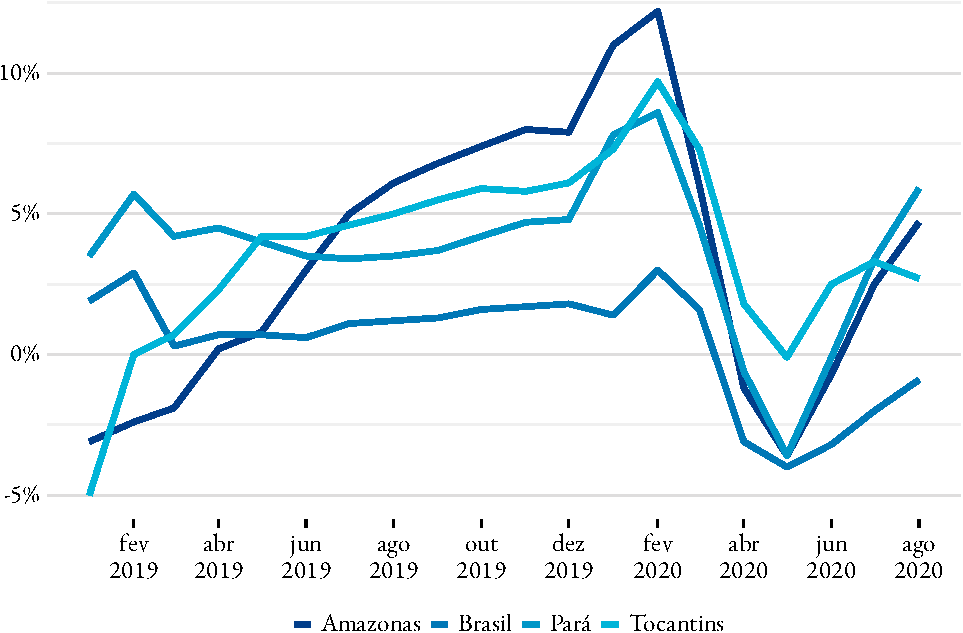
\includegraphics{rascunhoR_files/figure-latex/pmc_ibge-1.pdf}
    \source{IBGE}
    \end{subfigure}

    \begin{figure}[!h]
    \begin{subfigure}{\linewidth}
    \caption{Pesquisa Mensal de Serviços\label{fig:pms_ibge}}
    \subcap{Saldo Anual}
    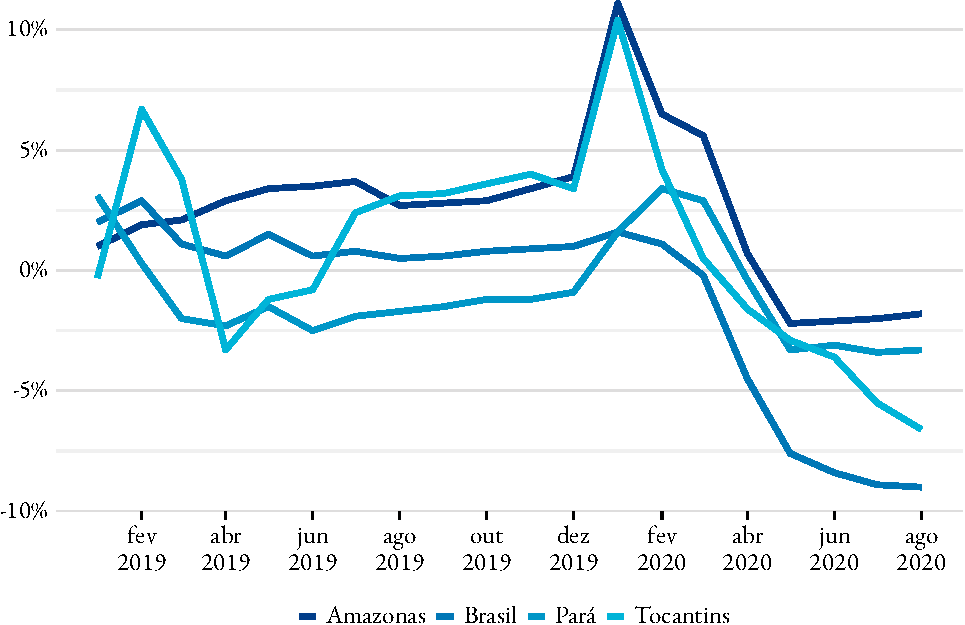
\includegraphics{rascunhoR_files/figure-latex/pms_ibge-1.pdf}
    \source{IBGE}
    \end{subfigure}

    \begin{figure}[!h]
    \begin{subfigure}{\linewidth}
    \caption{Expectativa de crescimento anual do PIB Nacional\label{fig:pib_expec}}
    \subcap{Saldo Anual}
    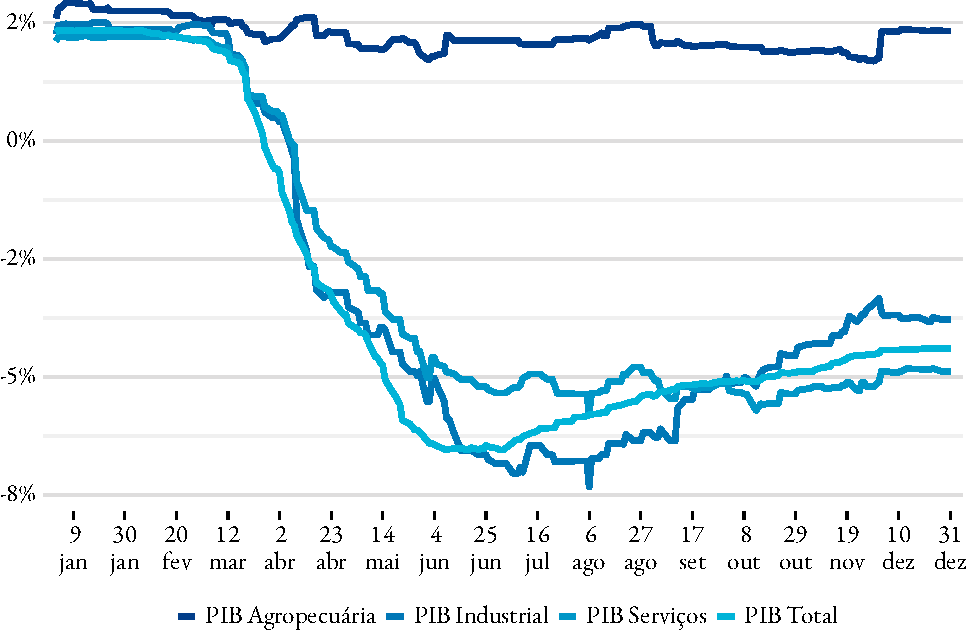
\includegraphics{rascunhoR_files/figure-latex/pib_expec-1.pdf}
    \source{SIDRA}
    \end{subfigure}

    \begin{figure}[!h]
    \begin{subfigure}{\linewidth}
    \caption{Variação trimestral do PIB pelo lado da demanda\label{fig:Variação trimestral do PIB - demanda}}
    \subcap{Com ajuste sazonal}
    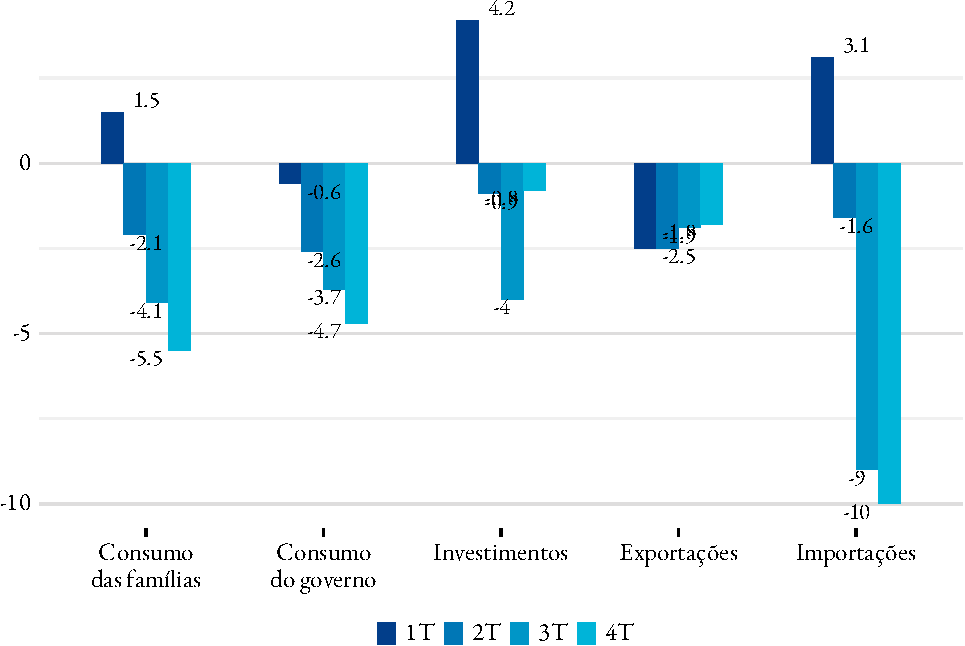
\includegraphics{rascunhoR_files/figure-latex/Variação trimestral do PIB - demanda-1.pdf}
    \source{IBGE}
    \end{subfigure}

    \begin{figure}[!h]
    \begin{subfigure}{\linewidth}
    \caption{Variação trimestral do PIB pelo lado da oferta\label{fig:Variação trimestral do PIB - Oferta}}
    \subcap{Com ajuste sazonal}
    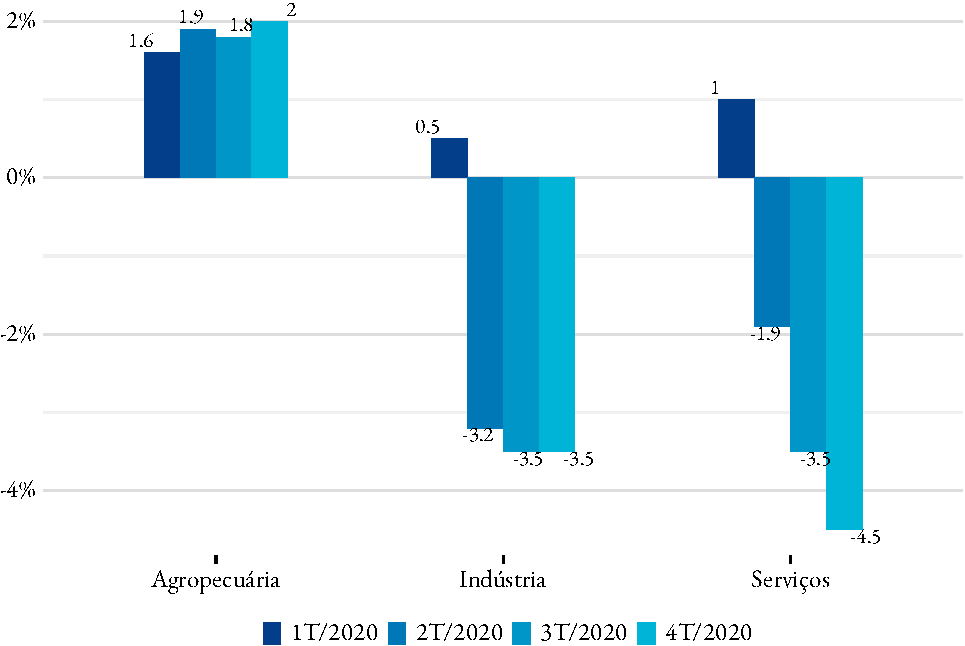
\includegraphics{rascunhoR_files/figure-latex/Variação trimestral do PIB - Oferta-1.pdf}
    \source{IBGE}
    \end{subfigure}

    \end{document}